%\section{Runtime Architecture}

\subsection{Runtime}
\label{sec:runtime}

\begin{figure}
		\centering
		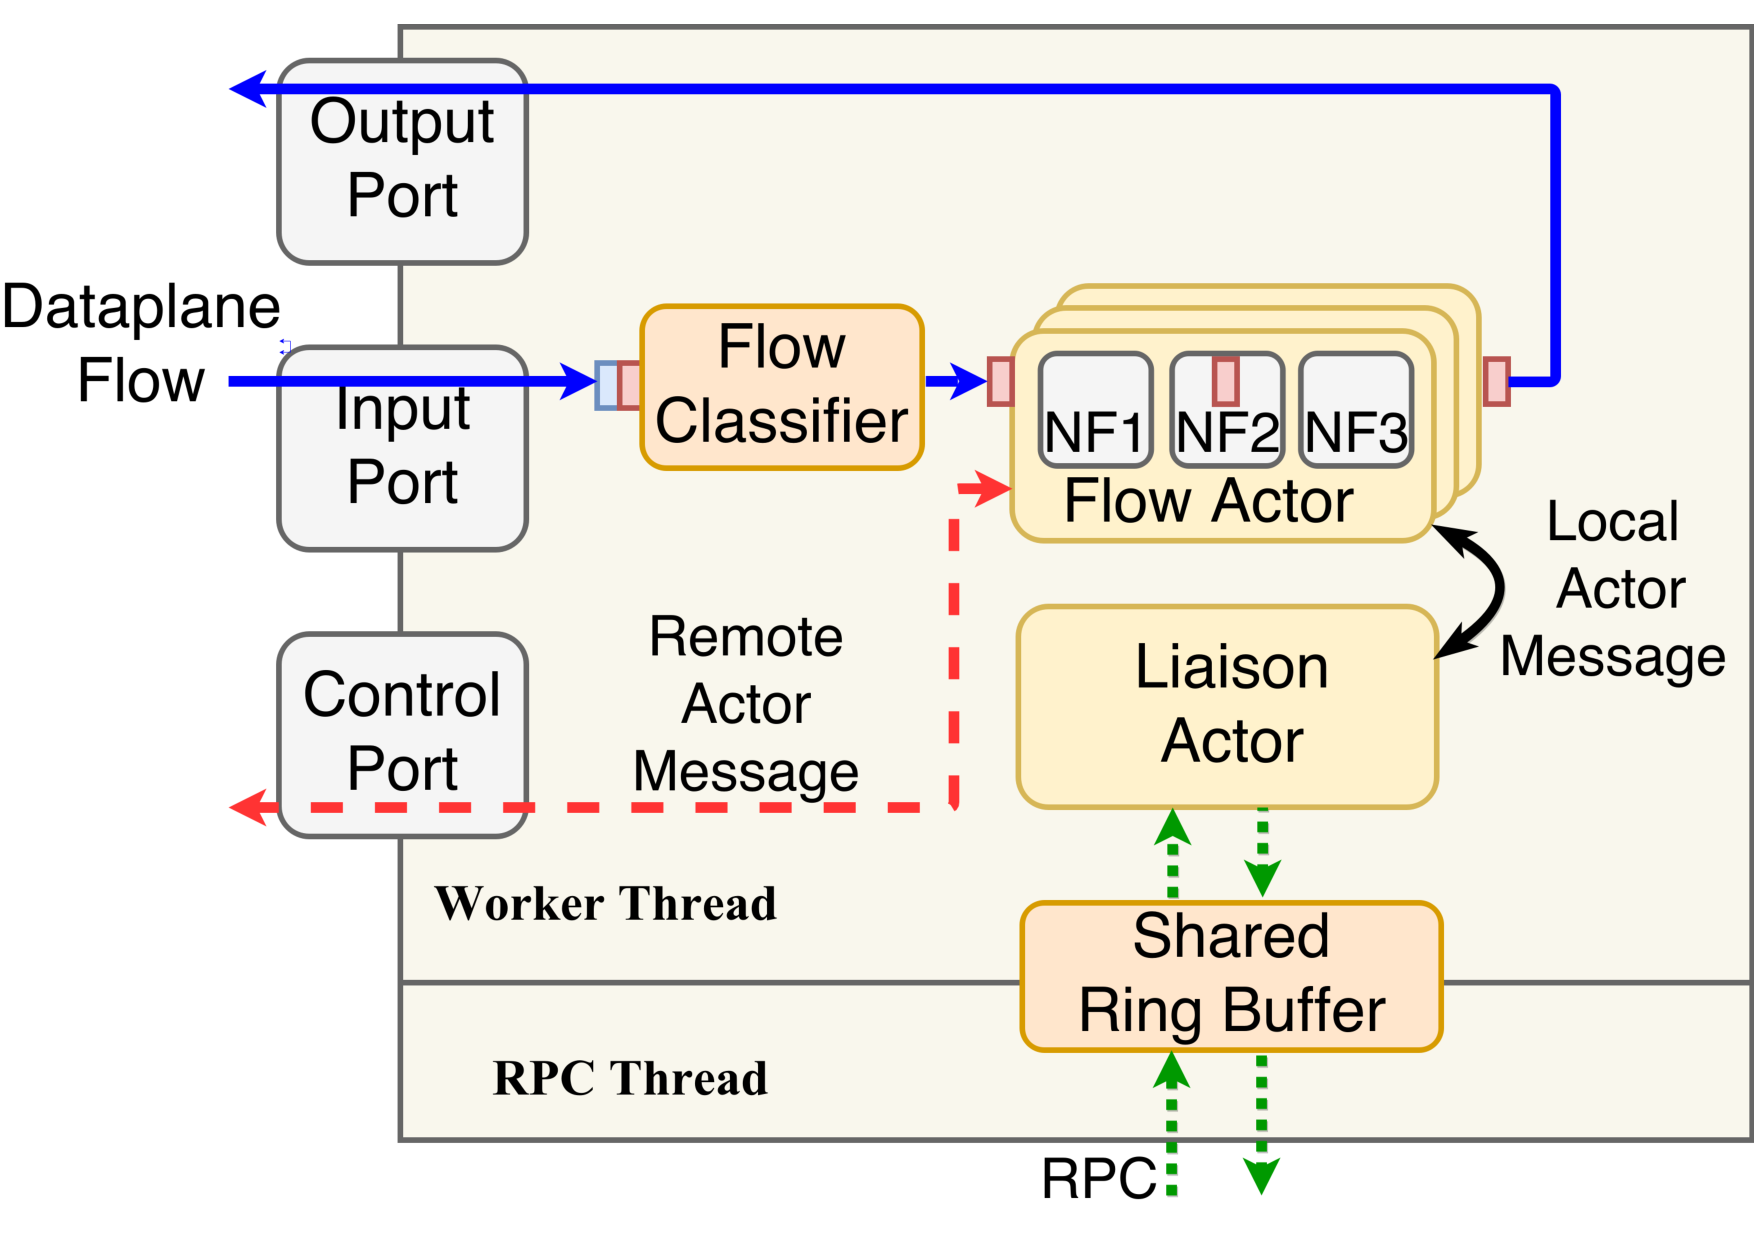
\includegraphics[width=\columnwidth]{figure/new-nfactor-runtime-arch.pdf}

		\caption{The internal structure of a runtime in \nfactor.}
\label{fig:runtime-arch}
\end{figure}

\nfactor~employs a carefully designed, uniform runtime system as the basic unit for deployment and scaling. %, does not appear in most existing work \cite{bremler2015openbox, gember2012stratos, palkar2015e2}. In existing NFV systems, the basic flow processing and scaling unit is an NF instance, which is a virtual machine or container hosting an instance of a NF. % and the NF instances are chained on the data-plane. % The flows must go through these NF instances in sequence.
 %The primary reason that we design such a runtime is to enable NFs/service chains to achieve failure resilience automatically without coordinator intervention, as the runtime provides a uniform communication channel to %network transparent abstraction \chuan{change this `network transparent' to a more accurate wording} to communicate and
 %exchange messages among each other, which are crucial for flow migration and replication.
  Within each runtime, we adopt the simple yet powerful design to create a micro execution context for each flow, and carry out %processing functions
  packet processing within the flow over its entire service chain inside the micro execution context. Especially, a dedicated flow actor is created for handling each flow, which loads all the NFs of the service chain that the flow should traverse, and passes the received packets of the flow to these NFs in sequence. We refer to this as the {\em one-actor-one-flow} design principle. Packet processing by NFs and operations to support flow migration and replication are all implemented as message handlers of the flow actor.


Fig.~\ref{fig:runtime-arch} shows the complete structure of a runtime. The input and output ports are used for receiving and sending flow packets from and to virtual switches. The control port %\chuan{no need to mention it here but directly introduce the case in loss avoidance part}as well as input and output ports,
is used for transmitting and receiving {\em remote actor messages}, exchanged for distributed flow migration and replication among actors running on different runtimes.  %and sent/received using DPDK.
 Input, output and control ports in each runtime are implemented with DPDK for high-speed raw packet transmission (Sec.~\ref{sec:implementation}).
 Input packets of dataplane flows are first sent to a flow classifier, which uses the 5-tuple of a flow (\ie, source IP address, destination IP address, transport-layer protocol, source port and destination port) to identify packets belonging to the same flow. %One flow actor is created for each new flow. Upon creation, the flow actor loads NFs of the service chain configured in the runtime.
 All packets of the same flow are sent to the same flow actor for processing. Other than flow processing, a flow actor participates in distributed flow migration and replication in response to certain actor messages. %, which processes them in sequence by passing them through NFs in the service chain.



%  \chuan{not clear what `allocate flow states' means. extract?} and xxx \chuan{describe what it does to facilitate flow migration and replication by rewriting the idea of the following sentence: `Besides service chain processing, the flow actor also provides an execution context for distributed flow migration and replication, in response to certain messages (Sec.~\ref{sec:resilience})'}.

Each runtime is configured with one specific service chain by the coordinator, and installs/initializes all the NFs of the service chain upon booting. Multiple flow actors may run concurrently in the same runtime, which all use the same service chain.  %and a number of carefully defined NF APIs, as given in Table \ref{table:api} in Sec.~\ref{sec:NFAPIs}, to allocate flow states for each NF and process packets across all the NFs.
 Based on the actor model, passing packets to a NF for processing in a flow actor is essentially just a function call. Hence only one copy of each NF needs to be loaded in a runtime, used by all flow actors.
%Each runtime can host one or multiple flow actors for flows passing through the same service chain that the runtime is configured with, depending on its resource availability and performance isolation requirements. In case of a multi-tenant NFV system, we can run actors processing flows of the same tenant on the same runtime, but those of different tenants on different runtimes, for better security and isolation.
 A worker thread schedules flow actors in a runtime: % a customized flow actor scheduler (Sec.~\ref{sec:implementation}),
  when a flow packet or a remote actor message arrives, the flow actor which is responsible for the flow that the packet belongs to, or is the destination actor of the remote message, is invoked; the packet or message is processed completely, before the scheduler moves on to handle the next packet/message, \ie, a run-to-completion scheduler \cite{199352}. %\chuan{cite papers mentioning this run-to-completion}.
 %An actor itself is a very lightweight one as millions of actors could be spawned in seconds \cite{chs-rapc-16}.


A runtime also consists of a RPC thread for receiving and responding to RPC requests from the coordinator, for basic system management operations (Sec.~\ref{sec:coordinator}). The RPC thread forwards received RPC requests to a {\em liaison actor} handled by the worker thread through a high-speed shared ring buffer.  The liaison actor coordinates with flow actors through {\em local actor messages} to carry out RPC requests from the coordinator. Having a dedicated thread for receiving RPCs saves the worker thread from potential context switches due to using kernel networking stack, expediting flow processing.
% The RPC thread and the worker thread share a ring buffer, used for relaying RPC requests received by the RPC thread to a liaison actor in the worker thread.
 %We use a high-speed shared ring buffer to achieve fast inter-thread communication \cite{dpdk}.
% flow actor initialization, flow migration and flow replication. %Flow actor and coordinator actor could directly exchanges local messages, or exchange remote messages through a reliable message passing module \cite{}.

%The worker thread routinely carries out the following tasks: (i) poll dataplane packets from input port, run the flow actor schedule to schedule flow actors to process these packets and send processed packets out from the output port; (ii) poll packets from the control port, reconstructspacket stream into remote actor messages and send the actor messages to the receiver flow actors; (iii) run the liaison actor to process RPC requests from the coordinator and dispatch %flow migration initiation
%messages to flow actors; (iv) fetch remote actor messages %from a queue that are enqueued
% produced by flow actors %during the execution of previous three tasks
%  and send them out from the control port. The input, output and control ports in each runtime are implemented with DPDK for high-speed raw packet transmission (Sec.~\ref{sec:implementation}).





\vspace{1mm}
\noindent {\bf Discussions on Runtime Design Choices.} Supporting only one service chain in one runtime avoids the overhead of installing many NFs per runtime and simplifies runtime management. Our one-actor-one-flow design facilitates fast flow migration, as compared to a few alternatives: (1) {\em One flow actor handles multiple flows.} It compromises the efficiency of flow migration, especially when multiple flows come from different virtual switch actors (Sec.~\ref{sec:virtualswitch}): the flow actor must synchronize responses sent from different virtual switch actors after their destination runtimes are changed, to ensure loss-avoidance during migration (Sec.~\ref{sec:migration}).
% adding overhead to flow migration process.
 (2) {\em One flow actor runs one NF}. Additional overhead is needed for chaining multiple flow actors to constitute a service chain, lowering packet processing speed. %Therefore, the one-flow-one-actor design achieves a sweet point in minimizing the actor processing overhead and improving the efficiency of flow migration protocol design.
 In addition, we use one worker thread to carry out all tasks including polling dataplane packets from input port and remote actor messages from control port, scheduling flow actors, send processed packets/messages out from output or control port,
and running the liaison actor to process RPC requests. Instead of using multiple worker threads, the single thread design guarantees a sequential execution order of flow actors, thus completely eliminating the need to protect message passing among flow actors by locks, and achieving higher efficiency.




%The alternative design to one-runtime-one-service-chain is to dynamically configure multiple service chains on a single runtime. Then due to the one-flow-one-actor design, we need to do an additional service chain selection, based on some pre-defined rules. This adds additional overhead to the flow actor processing and increases the complexity when managing the NFActor cluster, because the controller must populates the service chain rule dynamically to each runtime. With the one-runtime-on-service-chain design, if another service chain is needed, the system administrator could launch a new NFActor cluster and configure a different service chain to use.




%The runtime is designed as a single-worker-thread architecture to decrease the overhead of flow actors. A high speed NFV system may process millions of packets every second and migrates tens of thousands of flows. At such a high processing rate, message passing protected by shared lock in multi-threaded actor runtime system may incur a huge overhead and hurt the packet throughput.
%The runtime is configured with a specific service chain during the boot phase and initializes all the NF modules as specified in the service chain. When a flow actor is created, it loads these modules and uses the flow state allocation method \ref{table:api} to allocates all the
%To process flows across a service chain, during the initialization phase of the runtime, a service chain specifier is passed in to the runtime. The runtime then loads all the NF modules as indicated in the service chain specifier. When the flow classifier creates a new flow actor, the flow actor also loads these NF modules on the service chain and passes the input packet along the NF modules in sequence.

%The reason that the runtime is designed as a single-worker-thread program is because the multi-worker-thread design may not bring significant performance gain. In our initial prototype implementation, we use LIBCAF \cite{caf} library to construct flow actors. LIBCAF library creates multiple worker threads and schedules flow actors to run on these worker threads. Because LIBCAF completely conceals the internal interfaces of the worker threads, we have to create a dedicated polling thread to poll packet from the input port. Under this design, we find that the maximum throughput of a runtime does not increase when the number of LIBCAF worker thread increases, because the polling thread has always been a bottleneck. Therefore, we abandon the multi-worker-thread design and use a single worker thread to poll packets and schedule flow actors. To our surprise, this architecture turns out to work very well because it allows us to perform aggressive optimization of actor programming model \ref{}. In the mean time, we can still maintain the scalability of the system by launching more runtimes.

\subsection{NF APIs}
\label{sec:NFAPIs}

A clear separation of useful NF states from core processing logic of an NF is important to enable easy extraction of flow states during the runtime, that does not interfere with packet processing of the NF. We design a set of APIs for NFs to implement for this purpose, as listed in Table \ref{table:api}.

\begin{table}[!t]
%	\small
\centering
\caption{APIs for NFs in \nfactor}
\label{table:api}
\resizebox{\columnwidth}{!}{
\begin{tabular}{c|l}
\textbf{API}                                      & \multicolumn{1}{c}{\textbf{Usage}}                                                                                                                                                                                                         \\ \hline
nf.allocate\_new\_fs()                            & create a new flow state object \\
&for a new flow actor %, to be used for storing flow state
 \\ \hline
nf.deallocate\_fs(fs)                             & deallocate the flow state object \\
& upon expiration of the flow actor
\\ \hline
nf.process\_pkt(input\_pkt, fs)                   & process the input packet using \\
&the current flow state
\\ \hline
%nf.get\_migration\_target(cluster\_cfg, fs) & \begin{tabular}[c]{@{}l@{}}Query an NF using the current\\ cluster configuration and \\ flow state about which runtime this flow\\ actor should be migrated to\end{tabular} \\ \hline
\end{tabular}
}
\end{table}


%The APIs are  provided as three public methods for each NF to implement.
When a new flow actor is created to handle a new flow, it calls $allocate\_new\_fs()$ to create a flow state object for each NF in its service chain. %stores the flow state object in its internal storage.
Upon arrival of a new packet, the flow actor passes the packet and the flow state object to NFs for processing ($process\_pkt()$). Any changes to the flow state during NF processing is immediately visible to the flow actor. When the flow terminates, the flow actor expires and $deallocate\_fs()$ is called to deallocate the flow state objects. With these APIs, the flow actor always has direct access to the latest flow states, enabling it to sends them out upon flow migration or replication. %Therefore, the combination of the three methods servers as the basis for the transparent resilience in~\nfactor.

%\chuan{add the idea to flow migration section rather than exposign the API here} The fourth API $nf.get\_migration\_target(cluster\_cfg, fs)$ is used for checking where the NF would like the actor to migrate to, by passing the current cluster configuration and the current flow state. This enables the flow actor to actively migrate itself instead of waiting for migration initiation command sends from the controller \ref{}. This distributed design is the key to sparkle several useful applications, \ie, flow deduplication and reliable MPTCP subflow processing, which we will discuss in Sec.~\ref{sec:experiments}, that existing NFV systems based on centralized flow management cannot achieve. The flow actor should only call this method on the last NF in the service chain. Therefore NFs modules implementing this method should be placed on as the last NF in the service chain.

%These three methods are simple to use and properly generalize the structure of NFs that processes flow packets based on per-flow state. Using these three methods, we are able to create several representing NFs as shown in \ref{}.}

%The flow actor acquires the flow state of all the NF modules using the allocation API, and passes the packet across all the NF modules in sequence using the processing API.


To implement an NF in \nfactor, core processing logic of the NF should be ported to the actor model and the three APIs should be implemented. The implementation is relatively straightforward. We have implemented a number of NFs based on the model, such as IDS, firewall and load balancer (Sec.~\ref{sec:experiments}).


\subsection{Virtual Switch}
\label{sec:virtualswitch}

A virtual switch is a special runtime where the actors do not run a service chains but only a flow forwarding function. Following the one-actor-one-flow principle, a virtual switch creates multiple actors each to dispatch packets belonging to one flow. We refer to a flow dispatching actor in a virtual switch as a {\em virtual switch actor}.


A virtual switch learns runtimes that it can dispatch flows to through RPC requests its liaison actor receives from the coordinator, which include MAC addresses of the input ports of those runtimes. A virtual switch actor selects one of the runtimes to forward its flow in a round-robin fashion. We adopt a simple round-robin approach because the virtual switch must run very fast and a round-robin algorithm introduces the smallest overhead while providing satisfactory load balancing performance even in case of mixed long and short flows.

When a virtual switch actor receives an incoming packet, it replaces the destination MAC address of the packet to MAC address of input port of the chosen runtime, modifies the source MAC address of the packet to that of output port of the virtual switch, and then sends the packet out from the output port. When a virtual switch actor receives a processed packet for forwarding out, %is also used as a relay-point to the final destination of the dataplane traffic flows. By connecting the output ports of runtimes with the input port of a virtual switch
 it simply sends it to the output port, which uses pre-configured SDN rules to direct the packet to its final destination. %\chuan{check if this sentence is accurate}.


The architectural consistency of virtual switches and runtimes facilitates efficient flow migration and replication (Sec.~\ref{sec:management}). %The flow actor on a runtime can analyze the source MAC address of the incoming packets and determine which virtual switch this packet comes from. Then the flow actor can contact the virtual switch during flow migration and replication processes, to indicate change of the runtime that the respective virtual switch actor should dispatch packets to. This is done through sending a remote actor message to the virtual switch actor, which is further explained in Sec.~\ref{sec:resilience}. %remote control message exchanges with the virtual switch in the same way as message exchanges with other runtimes.
%Existing NFV management systems either rely on SDN switches \cite{gember2012stratos, gember2015opennf} to route flows from one NF to the next, or build a customized data-plane for inter-connecting different NF instances \cite{palkar2015e2}.
 A virtual switch in \nfactor~is lightweight, only responsible for dispatching flows to runtimes or outside, but not routing flows from one NF to anther as SDN switches in existing systems do \cite{gember2012stratos, gember2015opennf}.


%\chuan{describe how the virtual switches are used for receiving outgoing packets from runtime and send them to final destinations}



\subsection{Coordinator}
\label{sec:coordinator}

The coordinator in \nfactor~is responsible for basic cluster management routines, %(Sec.~\ref{sec:controller}),
\eg, launching and shutting down virtual switches and runtimes, updating latest cluster composition to the virtual switches and runtimes, monitoring workload of runtimes, %coordinating dynamic scaling,
 and participating in the initiation phase of flow migration and replication.
As compared to SDN controllers in the existing NFV systems \cite{gember2015opennf, rajagopalan2013split},
 the coordinator is much lightweight. % without involving in the entire flow migration and replication processes.
% Instead, flow migration and replication are handled in distributed fashion among flow actors, and only exploit the coordinator in the initialization phase.
The design of the coordinator is hence simplified (as a single thread module). % and the failure resilience of the system is improved, as the coordinator does not need to maintain complicated states associated with flow migration.



%The coordinator is responsible for launching new virtual switches and runtimes, monitoring the load on each runtime and executing dynamic scaling. Due to our distributed flow actor design, the coordinator only needs to participate in the initiation phase of flow migration and replication (Sec.~\ref{sec:resilience}). This differentiates \nfactor's coordinator with the controllers in existing NFV systems \cite{gember2015opennf}\cite{rajagopalan2013split}, which need to fully coordinate the entire flow migration process.


To deploy a service chain in \nfactor, the system operator first specifies composition of the service chain to the coordinator, as well as several rules to match input flows to service chains. The coordinator then launches a new virtual switch and a new runtime, configures the runtime with this service chain and installs several SDN rules that forward input flows using the service chain to the virtual switch. % and directs incoming flows using the service chain to the virtual switch.
Each runtime or virtual switch is assigned a global unique ID to ease management.  In \nfactor, a virtual switch is responsible for dispatching flows using the same service chain, to runtimes installed with this service chain. The virtual switches and runtimes handling the same service chain constitute a {\em cluster}. Flow migration and replication occur within a cluster. These design choices are made since they simplify system management and improve efficiency of both virtual switches and runtimes, for avoiding extra service chain selection for each flow.



The controller constantly polls load information from all the runtimes, and perform scaling out and in case of runtime overload or under-load %. When the coordinator detects that a runtime is overloaded, it scales up the cluster by launching a new runtime and configures the service chain on that runtime
(Sec.~\ref{sec:scaling}). The coordinator does not take care of the scaling of virtual switches. The scaling of virtual switch is offloaded to NIC hardware using Receiver Side Scaling (RSS) \cite{rss, jeong2014mtcp}, which is a static scaling method that requires the coordinator to configure a fixed number of virtual switches to match the number of receiver queues of the NIC.


The coordinator communicates with runtimes via a number of control RPCs exposed by each runtime, as summarized in Table \ref{table:rpc}. It uses $poll\_workload()$ to acquire the current load on a runtime. The coordinator updates cluster composition (including mac addresses of input/output/control ports and IDs of all runtimes and virtual switches in the cluster, and address of virtual switch(s) to forward process packets to) to all the runtimes and virtual switches using $notify\_cluster\_cfg(cfg)$.
%The cluster composition learned by different runtimes in a cluster do not have to be consistent because our flow migration and replication protocols perform safety checking by exchanging requests and responses to eliminate the inconsistency \chuan{check if this is true and revise accordingly}.
The last three RPCs are used to initiate flow migration and replication. After issuing these three calls, migration and replication are executed among runtimes without further involving the coordinator. %The use of RPC for coordinator to runtime communication decouples the execution of runtimes from the controller, therefore simplifying controller design.
%\chuan{briefly describe why you use RPC for coordinator to runtime communication.}


%\chuan{from Dr. Cui, the function style (C or C++) in table 2 should be the same as Table 1. Please change the style.}

%The coordinator also tells the liaison actor in a runtime the address of the virtual switch that the flow actors should send output packets to. The liaison actor made this information directly available to all the actors. During actor initialization phase, the actor saves the address information of the virtual switches that it is about to send output packets to. Whenever the actor finishes process the packet, it directly uses the information saved during initialization and send the output packet to the corresponding virtual switch.

\begin{table}[!t]
\centering
\caption{Control RPCs Exposed at Each Runtime}
\label{table:rpc}
\resizebox{\columnwidth}{!}{
\begin{tabular}{l|l}
Control RPC                                                                                   & Functionality                                                                                                                                              \\ \hline
poll\_workload()                                                                                   & \begin{tabular}[c]{@{}l@{}}Poll the load information \\ from a runtime\end{tabular}                                                                 \\ \hline
notify\_cluster\_cfg(cfg)                                                                         & \begin{tabular}[c]{@{}l@{}}Notify a runtime/virtual switch  \\the current cluster composition\end{tabular}                                                             \\ \hline
\begin{tabular}[c]{@{}l@{}}set\_migration\_target(runtime\_id, \\ migration\_number)\end{tabular} & \begin{tabular}[c]{@{}l@{}}Initiate flow migration. It tells \\ the runtime to migrate \\ migration\_num of flows to the \\ runtime with runtime\_id.\end{tabular} \\ \hline
set\_replicas(runtime\_id\_list)                                                                       & \begin{tabular}[c]{@{}l@{}}Set the runtimes with IDs  \\in runtime\_id\_list as the replica.\end{tabular}                                                                \\ \hline
recover(runtime\_id)                                                                          & \begin{tabular}[c]{@{}l@{}}Recover all the flows replicated \\ from runtime with runtime\_id.\end{tabular}                                                 \\ \hline
\end{tabular}
}
\end{table}
